\begin{savequote}[75mm]
OMG... Is that a neuron??
\qauthor{An Excited Grad Student}
\end{savequote}

\chapter{Systems for optical imaging in awake rats}
% INTRO
\newthought{Large-scale recordings} of hundreds and even thousands of neurons are becoming increasingly standard using electrophysiology \cite{NEUROPIXELS ETC} and optical imaging \cite{STRINGER}. With rapid advancements in genetic tools, hardware design, and computational power, we are in an unprecedented and exciting time to be studying neural circuits and behavior. For measuring neural populations in an awake animal, both of the main classes of techniques --- imaging and electrophysiology --- are extremely powerful, and choosing one or the other is highly dependent on the goals of the experiment. 

Electrophysiology provides the most direct access to neural activity, as it measures voltage changes with high temporal resolution, allowing for measurements of single spikes and sub-threshold activity \cite{REFREF}. It is also amenable to tethered or even wireless systems that allow animals to move about relatively freely, thus allowing a more naturalistic setting for studying neural circuits and behavior in the lab \cite{REFREF}. However, long-term access to a given neuron and the throughput of how many neurons can be recorded simultaneously is limited by the uncertainties in single unit isolation, the capacities of electronic components, and how many channels one can physically fit and successfully record from in a small animal. 

In contrast, optical approaches allow the same cells to be tracked for long periods of time, and simultaneous recording of large populations (hundreds to thousands) in the same animal. Optical imaging of neural activity relies on genetic tools that enable fluorescent indicators to be expressed in targeted cell populations. Standard approaches rely on tracking changes in calcium activity that occur in response to voltage changes in a neuron \cite{REFREF}. As such, the measured signal is slower and not a direct readout of neural activity, as measured by electrophysiology. Instead, calcium activity is measured by way of genetically-encoded fluorescent calcium indicators (GECIs)\cite{REFREF}, which fluoresce in response to calcium binding \cite{REFREF}. In transgenic animals, from fish\cite{REFREF} and flies\cite{REFREF} to mice\cite{REFREF} and marmosets\cite{REFREF}, these indicators can be expressed in a controlled manner, from sparse labeling \cite{REFREF} to pan-neuronal expression \cite{REFREF}. In the absence of a transgenic animal or in combination with one that expresses a different gene of interest, one can also use viral vectors, such as an adeno-associated virus (AAV) or lentivirus \cite{REFREF} for robust delivery of the GCaMP construct, and expression of the indicator remains robust and stable over at least several months \cite{REFREF}.

Physical access to deep or lateral parts of the brain is limited with optical methods, which typically rely on imaging the brain from directly above the animal's head. Many optical systems are bulky, making it quite difficult to record from freely moving animals. While electrodes can be inserted deep and at any angle into the brain, optical access to deeper brain structures sometimes requires removing superficial layers\cite{REFREF}, or using mirrors to direct the light path in clever ways while keeping the collection system above the animal \cite{REFREF prism}. Head-mounted optical systems allow for cellular resolution imaging in freely moving animals \cite{REFREF miniscope, Helmchen2001, Sawinski2009}, and high-photon-count imaging (\textit{e.g.}, >3 photon \cite{REFREF}) improve optical access to deeper brain structure

However, the gap between the two methods continues to get smaller, as technological advancements offer improvements to the challenges each face. There continue to be major technical advances in electrophysiological approaches, such as high-density electrode arrays \cite{REFREF} and computational methods for processing high channel count data and verifying chronic access to specific cells \cite{REFREF}. For imaging, 

Each generation of calcium indicators has proved increasingly more powerful, \textit{e.g.}, higher signal-to-noise (SNR), multi-color alternatives, and higher temporal resolution \cite{Akerboom2012OptimizationImaging, Chen2013UltrasensitiveActivity, REFREF}. Several groups \cite{REFREF, Adam Cohen, etc} have been developing voltage-sensitive indicators, which have the potential to combine the advantages of spatial and genetic access provided by optical methods with the more direct signal and higher temporal resolution of electrophysiology. High-photon-count imaging (\textit{e.g.}, >3 photon \cite{REFREF}) improve optical access to deeper brain structure

Today, one of the greatest advantages of optical imaging is cellular resolution access to large swaths of the brain. To be able to visualize single neurons as a population in awake animals is immensely powerful, especially in concert with sophisticated manipulation techniques, such as multi-channel optogenetics \cite{REFREF}, holographic light stimulation \cite{REFREF}, and genetically-defined targeting of specific populations of cells. In combination, these features allow one to measure and manipulate the same neurons in awake, behaving animals across large numbers of stimuli and trials over the course of weeks and months. In contrast, conventional acute single-unit microelectrode recordings are limited by the time that a single cell can be isolated (usually only one or a few hours). Even the best chronic preparations face difficulties holding isolated cells over very long time periods, and it is difficult to be absolutely confident that the same cell is isolated across days, especially given that nearby cells are often thought to have similar response properties.

Nonetheless, head-fixed preparations afford certain experimental advantages, such as restrained movement, precise stimulus control, and longitudinal studies that can track the same neurons over long timescales. Although a large body of scientific research relies on the rich behavioral repertoire of rats, it has not been possible to fully leverage recent developments in optical imaging and molecular and genetic tools, as has been done with great success in smaller animals like mice. 

Within the past decade, there have been significant advances for using rats as a model in systems neuroscience. In particular, Scott \textit{et al.} developed a method for training rats in voluntary fix themselves in a two-photon system, which allowed for cellular resolution imaging in awake, behaving rats \cite{Scott2013}. However, voluntary head-fixation can be difficult and time-intensive, requiring significant training in order just for the imaging, which significantly limits how much control the experimenter can have over the time course of the study. More recently, the same group also created a transgenic rat expressing GCaMP in all neurons, and demonstrated the feasibility of recording population dynamics in awake, freely moving rats \cite{Scott2018ImagingMacroscope}. 

Miniature head-mounted two-photon microscopes offer an alternative to head-fixation during in vivo imaging \cite{Helmchen2001, Piyawattanametha2009, Sawinski2009}. Such techniques can be powerful for measuring neural activity in a wide range of naturalistic behaviors \cite{Sawinski2009}, but the technical difficult of using these miniaturized microscopes has limited their use as a standard tool in neuroscience \cite{Kerr2012}. Furthermore, many other in vivo imaging technologies are difficult to miniaturize, preventing their use as head-mounted devices. 


% FIGURE 2.1 Rat visual areas
\begin{figure}[t!]
    \includegraphics[width=\textwidth]{figures/chapter_2/rat_visual_areas.pdf}
    \vspace{.1in}
    \caption[Visual areas in the rat]{Visual areas in the rat. \textbf{A.} Lateral view of visually responsive areas identified by electrophysiological mapping of retinotopic preference. \textbf{B.} Flattened representation of lateral visual areas, with targets of the present study highlighted in REFREF. 
    \label{fig:rat_visual_areas}}
\end{figure}

%% % What has been done, and what's missing  ---------------------------
Rat visual cortex contains several areas, the largest of which is striate or primary visual cortex, or V1, with additional extrastriate areas surround V1 \cite{Espinoza1983RetinotopicRat, Sereno1991} (Figure~\ref{fig:rat_visual_areas}). Adding to this challenge, in rats, areas V1, LM, LI, and LL lie along the medial-to-lateral axis at the posterior edge of the brain, extending well beyond the lateral bone ridge (Figure\ref{fig:rat_visual_areas}). 

Almost all of our knowledge about rat visual cortex comes from electrophysiology studies. To date, the only area of visual cortex to be imaged from in rats is primary visual cortex, or V1, from intrinsic signal \cite{Gias2004} to single-photon \cite{Scott2018ImagingMacroscope} and two-photon \cite{Ohki2005, Greenberg2008} imaging. Building off of this work, we developed a method for cellular-resolution imaging of large FOVs in awake, head-fixed rats with the ultimate goal of chronic neural imaging across lateral extrastriate cortex. 

% %%%%%%%%%%%%%%%%%%%%%%%%%%%%%%%%%%%%%%%%%%%%%%%%%%%%%%%%%%%%%%%%
% Scopes + tool development  
% %%%%%%%%%%%%%%%%%%%%%%%%%%%%%%%%%%%%%%%%%%%%%%%%%%%%%%%%%%%%%%%%
Optical imaging approaches allow the same field-of-view (FOV), and with multiphoton imaging, the same cells, to be imaged across multiple sessions. Our approach aimed to combine head-fixation in awake rats, optical access to multiple brain areas, and precise re-positioning for long-term studies of chronically implanted animals. Several major challenges that needed to be addressed were:  1) accessibility of large FOVs over the extreme, lateral edge of the rat skull, 2) implant stability against the significant mechanical forces that awake rats are able to apply, and 3) motion artefacts due to large displacements in moving rats. 

% window surgery --------------------------------------
\section{Cranial windows for chronic imaging in awake rats}
For calcium imaging, we relied on viral expression of GCaMP across an area of cortical space covering about 4-6mm. A region of this size was large enough to contain multiple visual areas in the rat, based on known cortical extents of extrastriate areas (see Figure\ref{fig:rat_visual_areas}). Since the transgenic GCaMP rat \cite{Scott2018ImagingMacroscope} had not been developed yet, it was important to calibrate the correct volume, titre, and injection method for consistent, widespread expression of the virus throughout the window (see Methods). 

% Figure: Cranial window + implant
\begin{figure}
    \includegraphics[width=\textwidth]{figures/chapter_2/surgery_steps.pdf}
    \vspace{.1in}
    \caption[Chronic cranial window]{Implant of chronic cranial windows for GCaMP imaging. \textbf{a.} Exposed cortical surface and craniotomy during a microinjection of AAV-GCaMP. Blue, dye used to visualize spread (see Methods) \textbf{b.} Bright-field view of a cranial window REFREF. \textbf{c.} Fluorescent view of GCaMP expression in the cranial window shown in \textbf{c} REFREF TODO.
    \label{fig:surgery_steps}}
\end{figure}

% Headplate assembly
We adapted a surgical protocol for chronic cranial windows in mice \cite{Goldey2014} that optimized implant adhesion and long-term viability for optical access, even against significant forces applied by awake rats (see Methods, REFREF). Moreover, in order to access  lateral visual areas while keeping the rat’s head and body in a relatively natural resting position, our approach was to tilt the imaging plane relative to the animal’s head. This meant implanting the headplate at an angle that matched that of the objective. 

% Figure: Headplate and holding the rat
\begin{figure}
    \includegraphics[width=\textwidth]{figures/chapter_2/headplate_schematic.pdf}
    \vspace{.1in}
    \caption[Headplate design and assembly]{Headplate design and assembly. \textbf{a.} Exposed cortical surface and craniotomy during a microinjection of AAV-GCaMP. Blue, dye used to visualize spread (see Methods) \textbf{b.} Bright-field view of a cranial window REFREF. \textbf{c.} Fluorescent view of GCaMP expression in the cranial window shown in \textbf{c} REFREF TODO.
    \label{fig:headplate_schematic}}
\end{figure}

For the implant itself, we leveraged the high precision afforded by kinematic mounts to design custom titanium headplates that could be mounted at steep angles while preserving the capacity for precise re-positioning (Figure\ref{fig:headplate_schematic}). The headplates contained three semi-spherical grooves that mated with stainless steel ball bearings mounted to an aluminum post on the imaging platform. The headplate mated with a steel post designed to be strong enough to hold the animal stably, while keeping the view to the stimulus monitor unobstructed on one side of the animal, and on the contralateral side, sufficiently clear for the objective. Implanted animals were stably positioned at the farthest angles tested (40-45 degrees, where 0 degrees is parallel to ground, or flat on the skull).  

% Figure: Experimental pipeline
\begin{figure}
    \includegraphics[width=\textwidth]{figures/chapter_2/experimental_pipeline.pdf}
    \vspace{.1in}
    \caption[Experimental pipeline]{Headplate design and assembly. \textbf{a.} Exposed cortical surface and craniotomy during a microinjection of AAV-GCaMP. Blue, dye used to visualize spread (see Methods) \textbf{b.} Bright-field view of a cranial window REFREF. \textbf{c.} Fluorescent view of GCaMP expression in the cranial window shown in \textbf{c} REFREF TODO.
    \label{fig:experimental_pipeline}}
\end{figure}

% Habituation + shaping
Rats are much larger than mice, so a key challenge was to prevent awake rats from ripping themselves out of their implants and keeping the FOV stable enough for cellular resolution imaging. To reduce prohibitively large motion artefacts from rats resisting head-fixation, we developed a shaping procedure to habituate rats for multi-hour sessions (Figure\ref{fig:experimental_pipeline}). Briefly, rats were placed in a red, transparent cylinder also used as enrichment in their home cages, and over the course of several days (REFREF ~3-4 days) animals were given decreasing doses of sedative and increasingly long habituation sessions (REFREF  gradually increasing from 30 minutes to 3 hours). 


% WIDEFIELD --------------------------------------
% Figure: widefield_scope
\section{A tandem-lens macroscope for wide-field imaging}
To optically map extrastriate areas of rat visual cortex for the first time, we developed a tilting tandem-lens epifluorescence macroscope\cite{Ratzlaff1991} for mapping the visual areas accessible in a given cranial window (Figure\ref{fig:widefield_scope}). Specifically, we needed a large field-of-view (FOV) that could capture the full extent of the window (4-5$mm$). In order to ensure robust mapping with high signal-to-noise, we also needed a sufficiently shallow depth of field for avoiding out-of-focus artefacts (\textit{i.e.}, good axial resolution).

% Figure:  Widefield epi setup
\begin{figure}
    \includegraphics[width=\textwidth]{figures/chapter_2/widefield_scope.pdf}
    \vspace{.1in}
    \caption[Tandem-lens macroscope]{Wide-field imaging of rat visual cortex. \textbf{a.} Schematic of the tandem-lens macroscope. \textbf{b.} Photograph of a rat during a mapping session. REFREF TODO.
    \label{fig:widefield_scope}}
\end{figure}

The macroscope combined two $50mm$ lenses in reverse configuration with a CCD camera, with the whole assembly mounted on a rotating plate (Thorlabs). The plate itself was mounted on a translating stage that allowed travel in all four directions with manual micrometers. For epifluorescence illumination, we used a 470 nm LED filtered and reflected by a long-pass dichroic mirror, and emitted fluorescence was filtered and captured at an imaging rate of 25Hz. A full-resolution (656x492, $9.9um$ pixels) image was taken of the vasculature at the surface of the brain for coregistration with later two-photon imaging sessions. For functional imaging, we focused below the surface to $500um$. 

% 2p setup --------------------------------------
\section{A tiltable 2-photon microscope for cellular resolution}
% Figure: 2p_schematic (beam path, 2p schematic, face-camera, schematic of whole thing?)
% Figure:  2p_fovs, separate (Imaging modes:  compare 2x, 4x, also show dual channel).
% Figure:  experimental_pipeline
For cellular resolution imaging, we created a custom, two-photon excitation microscope especially designed for recording from all visual areas in an awake behaving rat. A key feature of this microscope is its ability to pivot about the focal point of the microscope objective --- the microscope can be tilted to any orientation required to access lateral cortical areas while keeping the animal in a natural, unrotated position (Figure\ref{fig:2p_schematic}). Meanwhile, the body of the microscope was constructed so as to allow ample space for the animal's body while maintaining over 180º of unobstructed viewing angle for a head-fixed animal.

% Figure:  2p schematic
\begin{figure}[t!]
    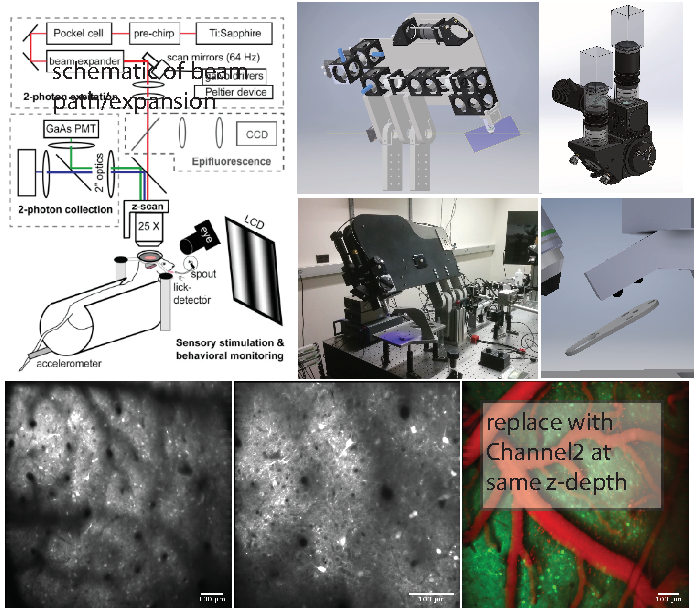
\includegraphics[width=\textwidth]{figures/chapter_2/2p_schematic.pdf}
    \vspace{.1in}
    \caption[Tilting two-photon microscope]{Tiltable 2-photon microscope. \textbf{a.} REFREF.
    \label{fig:2p_schematic}}
\end{figure}

The microscope was built on a tilting platform that allows any region of visual cortex to be targeted, including far lateral regions. It supports dual-channel imaging (red and green), allowing for either two functional channels (\textit{e.g.}, nuclear-localized red GECIs with green GECIs outside the nucleus), or, one anatomical channel (blood vessels filled with SR101, a fluorescent dye) for registering volumes and motion correction with the other, functional GCaMP channel (Figure\ref{fig:2p_schematic}). Attached is an epifluorescence imaging path for intermediate-sized FOVs if retinotopic validation is needed at an intermediate level (Figure\ref{fig:2p_schematic}). 

We created two imaging modes for the microscope (Figure\ref{fig:2p_schematic}). The first is a more standard imaging field (up to $0.5mm$x$1mm$), with high cellular resolution (~$1um$x$1um$x$2um$ estimated point spread function, measured with a 16x/0.8NA Nikon objective). The second mode is a much larger FOV (up to $1mm$x$2mm^2$) with slightly lower, albeit still single-cell resolution (~$2um$x$2um$x$12um$ estimated point spread function). This second mode provides access to the majority of a given visual area in the rat brain, and in some cases, multiple areas simultaneously. 

% Reaching our dreams
% Figure:  Multi-day imaging (2 example rats)
The kinematic mount for our titanium headplate was not only designed to hold the animal stable, but importantly, to allow precise re-positioning of animals from day to day. In combination with blood vessel landmarks and the unique layout of fluorescent, GCaMP-expressing cell bodies in a given field-of-view in 3-dimensional space, this precise re-fixation allowed us to rapidly relocate the same cells across sessions (Figure\ref{fig:multiday_imaging}). It is difficult in any GCaMP-labeled brain to get the same exact population on each day, due to differences in baseline activity and generic neural tissue movement that occurs across hours. However, the majority of well-labeled cells combined with scanning in depth enabled good matching across sessions, as quantified by REFREF. 

% Figure:  2p, multiday_imaging
\begin{figure}[t!]
    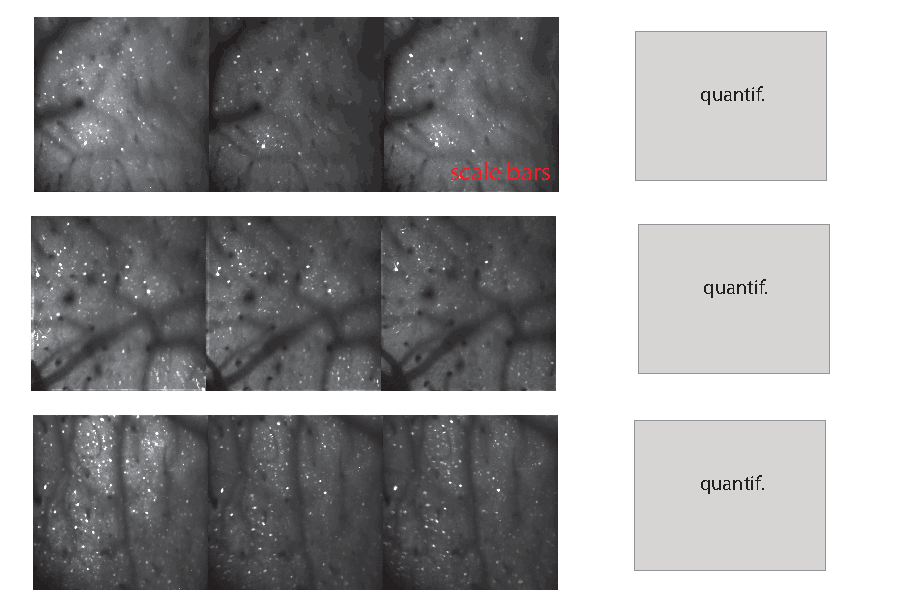
\includegraphics[width=\textwidth]{figures/chapter_2/multiday_imaging.pdf}
    \vspace{.1in}
    \caption[Multi-day imaging]{Imaging the same site across days. \textbf{a.} REFREF.
    \label{fig:multiday_imaging}}
\end{figure}

% Figure: 2-area imaging
% REFREF TODO?

% Pupil/face-tracking REFREF TODO.
Finally, since we were recording neural activity in awake animals, it was critical to monitor their behavior and other facial movements. Arousal states and locomotion modulate neural activity in ways that are unrelated to the task at hand or stimulus being shown to the animal. Moreover, particularly for vision experiments, the characterization of visual cortex also depends on knowing and controlling where stimuli fall on the retina. To track eye movements and all other visible behaviors, we simultaneously recorded high-resolution images using an IR-illuminated camera system (Allied Vision, MantaXX REFREF) mounted on one side of the animal. Behavior acquisition was synced frame-by-frame to two-photon imaging acquisition to track and align behavioral features, e.g., pupil dynamics, oral movements, etc., to all imaging data (Figure\ref{fig:2p_schematic}, TODO REFREF).

% %%%%%%%%%%%%%%%%%%%%%%%%%%%%%%%%%%%%%%%%%%%%%%%%%%%%%%%%%%%%%%%%
% Functional mapping
% %%%%%%%%%%%%%%%%%%%%%%%%%%%%%%%%%%%%%%%%%%%%%%%%%%%%%%%%%%%%%%%%
\section{Functional identification of visual areas}
% Figure: Stimulus protocol + example maps + responses
% Figure:  Area segmentation and boundaries
% Figure:  2p retino/neuropil version

Visual areas are retinotopically arranged --- each area contains a representation of the visual field called a retinotopic map, where nearby positions in physical space are represented by nearby cells on the retina, and this spatial arrangement is preserved from one part of the visual system to the next \cite{REFREF}. Conveniently, nearby visual areas have predictable ``reflections'' of retinotopic space at area boundaries. As such, distinct visual areas can be functionally identified by these mirror reflections in the representation of the visual field. To date, the only area of visual cortex to be imaged from in rats is primary visual cortex, or V1, from intrinsic signal \cite{Gias2004} to single-photon \cite{Scott2018ImagingMacroscope} and two-photon \cite{Ohki2005, Greenberg2008} imaging.

% Figure:  retino_mapping (WF)
\begin{figure}
    \includegraphics[width=\textwidth]{figures/chapter_2/retino_mapping.pdf}
    \vspace{.1in}
    \caption[Retinotopic mapping]{Identifying visual area boundaries. \textbf{a.} REFREF.
    \label{fig:retino_mapping}}
\end{figure}

For fast acquisition of retinotopic maps, we used Fourier-based calcium imaging\cite{Kalatsky2003} (Figure\ref{fig:retino_mapping}). This approach is less time-consuming (<10 minutes) than traditional event-based paradigms in which discrete positions on a monitor are stimulated one-by-one across repeated presentations to average over noisy responses, which can take many minutes or longer. In a standard Fourier-based mapping experiment, a moving bar cycles across the screen several times at at particular frequency. The position on the screen to which a given pixel best responds corresponds to a particular part of the bar's cycle, \textit{i.e.}, the phase of response at the stimulation frequency, while how strongly a pixel responds is given by the magnitude of its response at that frequency. Calculate the phase and magnitude of response for each pixel generates a 2D map of phase and magnitude. The phase map is the retinotopic map, which we use to delineate area borders base on the mirror reflections (see Figure\ref{fig:retino_mapping}), and the magnitude map can be used to filter out unresponsive pixels (and thus, remove phase values that are meaningless). 

Visual stimuli were presented using custom Python scripts (see Methods) on a large LCD monitor, which was centered in front of the left eye to span the animal's visual field left visual field (~177$^{\circ}$ of visual angle along azimuth, 67$^{\circ}$ along elevation). The mapping protocol consisted of a periodic, moving bar stimulus\cite{Kalatsky2003, Marshel2011} presented to the (left) eye contralateral to the cranial window. The bar was either a white bar drifting over a black background or an apertured bar containing a random subset of natural scene images drifting over a gray background. We did not find an clear difference between the two bar types, but qualitatively, the latter seemed quite reliable, so we primarily used the natural scene bars for the mapping sessions. The bar was presented at 0.13 Hz along the azimuth and elevation axes, for a total of 2 (downward, rightward) or 4 (downward, rightward, leftward, upward) conditions. A total of 4-5 repetitions of 10 cycles each were acquired for each direction. 

Though we tried both intrinsic imaging and calcium imaging, we found that calcium imaging in lightly anesthetized animals was the most reliable for quickly identifying the boundaries of each visual area within a given cranial window. This precluded the need for motion correction and multiple repeated session due to animal movement, as mapping was typically done prior to habituation (see Figure\ref{fig:experimental_pipeline}). Specifically, we found that with light levels of anesthesia (minimal isofluorane, 0.5-1\%, and a small dose of choloprothixene, $2mg/kg$ REFREF), such that animals woke up alert immediately after the isofluorane nose cone was removed, we were able to acquire strong neural signal without needing motion correction for processing the maps.

We observed smooth retinotopic maps in  V1, LM, and LI, as well as in surrounding areas, such as AL and RL across rats (Figure\ref{retino_mapping}). In some animals, the cranial window spanned all three areas, but in most cases, only one or two areas were accessible with sufficient GCaMP expression for population imaging at cellular resolution (V1: REFREF rats across REFREF imaging sites, LM: REFREF rats across # imaging sites, Li: REFREF rats across REFREF imaging sites, see Methods).

% Area segmentation
To segment the visual areas, we used an established method that converts the phase map into a sign map based on the gradient of the image to determine the direction reversals, which are the area boundaries\cite{Garrett2014, Zhuang2017}. We excluded any animals that had ambiguous maps (see REFREF\ref{fig:REFREF} for examples of clear and ambiguous maps). Across animals, there was some variability in which visual areas were contained within the cranial window and the patchiness of expression due to inconsistent viral spread or injections. Patchy expression presented a challenge to a fully automated segmentation approach, for example, by splitting visual areas that should be continuous, or assigning an area where viral expression and signal was quite poor. All maps were thus inspected by eye, and patch merging and smoothing parameters were manually adjusted based on visual sign consistency, size and orientation of a given visual area relative to surrounding areas (since all windows captured minimally 1-2 mirror reflections), and comparison with movies of the imaging session, which allowed direct visualization of the stimulus traveling on the cortical surface. 

\section{Coregistration and validation of 2-photon FOVs}
% Blood vessel coregistration
% Figure: 2p_retino?

% % Figure:  Coregistration & 2p_retino
% \begin{figure}
%     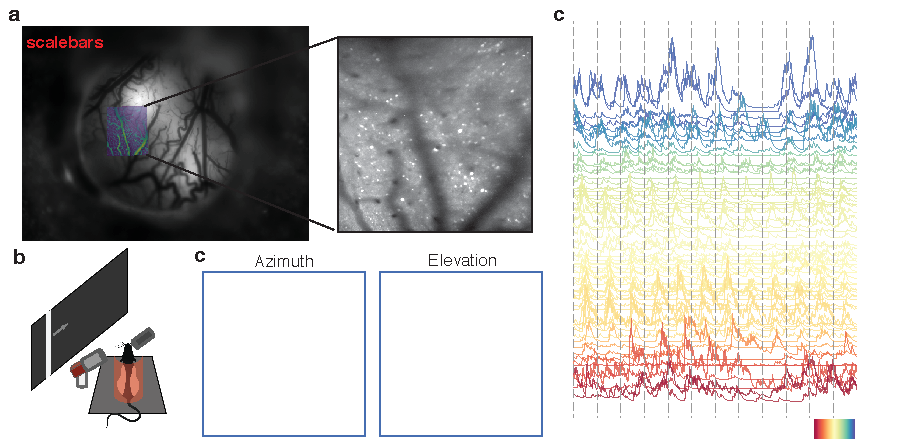
\includegraphics[width=\textwidth]{figures/chapter_2/2p_retino.pdf}
%     \vspace{.1in}
%     \caption[Coregistration and area identification in 2p]{Coregistration and area identification in 2p . \textbf{a.} REFREF.
%     \label{fig:2p_retino}}
% \end{figure}

We used the wide-field area maps to determine which visual areas in a given window we should image for two-photon imaging. At the start of a given two-photon session, we targeted sites of interest by eye, using blood vessel patterns relative to the area boundaries identified by the wide-field maps. In order to register the two-photon maps to the wide-field maps, we acquired an anatomical volume at the start of each session. This was a surface-level z-stack that captured fiduciary markers in both channels: while the green channel was always used for functional runs (GCaMP), we used the red channel to acquire images of blood vessels filled with a temporary fluorescent dye that was injected at the start of each session (see Methods). If blood vessel images were unavailable, the green channel could be used for registration. 

Two-photon blood vessel images were matched offline to the high-resolution images we took of the brain surface in each wide-field mapping session (Figure\ref{fig:retino_mapping}). We selected matching points between the two views based on uniquely identifiable blood vessels present in both images, then used these points to identify a transformation matrix to warp one into the other.

% % 2p retinotopy
% Using the same stimulus protocol as used in the macroscopic mapping, we then mapped retinotopic preferences at single-cell resolution with two-photon calcium imaging. We observed retinotopic maps across visual axes of elevation (ventral-dorsal) and azimuth (nasal-temporal) in all targeted FOVs for areas V1, LM, and LI (Figure\ref{fig:retino_mapping}). 

%%%%%%%%%%%%%%%%%%%%%%%
% While previous studies have shown used coarse retinotopy to identify the areas in which they were recording, the fine-scale retinotopic organization of cell bodies in any extrastriate area remains unknown. To characterize retinotopic preferences at single-cell resolution, we used the same phase-encoding Fourier paradigm used in wide-field mapping with two-photon calcium imaging.


% % Retino scatter
% Cell bodies exhibited a coarse-scale retinotopic organization. However, retinotopic preferences of neighboring cells were disordered and deviated from the surrounding neuropil in V1, LM and LI {\fig:Figure1f, REFREF, Supplemental 2.2, 2.3, stats REFREF}, consistent with findings in mouse visual cortex \cite{Liang2018, Andermann2011, Marques2018}. Single sweeps of the stimulus evoked robust responses in individual cells. 


% We found an asymmetric expansion of spatial representation along the elevation axis in all areas tested (Figure\ref{fig:2p_retino}). There was a ~2-fold increase in cortical magnification along the visual axis of elevation versus azimuth (REFREF paired t-test, V1: p=#, LmL p=#, Li: p=#). 